%----------------------------------------------------------------
%
%  File    :  chapter6.tex
%
%  Authors : Michael Fuska, FH Campus Wien, Austria
%  Created : 13 Feb 2016
%
%  Changed :  
% 
%----------------------------------------------------------------


\chapter{Analyse und Ergebnisse}
\label{ch:Ergebnisse}

%------------------------------------------------------------------------------
%------------------------------ Analysen zur Frage 1

\section{Welche Faktoren sind für die Sicherheit und die Vertrauenswürdigkeit eines iOS Device ausschlaggebend}
\label{sec:Frage1}

\begin{table}[htp!]
    \begin{center}
        \begin{tabular}{|p{30mm}|p{27mm}|p{12mm}|p{10mm}|p{18mm}|p{2cm}|p{15mm}|} \hline
            \textbf{iOS Device} & \textbf{Verkaufsstart} & \textbf{initial iOS} & \textbf{last iOS} & \textbf{Secure Enclave} & \textbf{Prozessor}  & \textbf{\#Tage JB} \\ \hline
            \textbf{iPhone} & 29.06.2007  & 1.0 & 3.1.3 & nA & Samsung SSL8900 & 11\\ \hline
            \textbf{iPhone 3G} & 11.07.2008 & 2.0 & 4.2.1 & nA & Samsung SSL8900 & 9\\ \hline
            \textbf{iPhone 3GS} & 19.06.2009 & 3.0 & 6.1.6 & nA & Samsung SSL8920 & 14\\ \hline
            \textbf{iPhone 4} & 01.08.2010 & 4.0 & 7.1.2 & nA & Apple A4 & 38 \\ \hline
            \textbf{iPhone 4s} & 20.01.2012 & 5.0 & 9.3.2 & nA & Apple A5 & 98 \\ \hline 
            \textbf{iPhone 5} & 21.09.2012 & 6.0 &  9.3.2 & nA & Apple A6 & 136 \\ \hline
            \textbf{iPhone 5c} & 22.12.2013 & 7.0 & 9.3.2 & nA & Apple A6 & 93 \\ \hline
            \textbf{iPhone 5s} & 22.12.2013 & 7.0 & 9.3.2 & A & Apple A7 & 93 \\ \hline
            \textbf{iPhone 6} & 19.09.2014 & 8.0 & 9.3.2 & A & Apple A8 & 33\\ \hline
            \textbf{iPhone 6 Plus} & 19.09.2014 & 8.0 & 9.3.2 &  A & Apple A8 & 33\\ \hline
            \textbf{iPhone 6s} & 25.09.2016 & 9.0 &  9.3.2 & A & Apple A9 & 19\\ \hline
            \textbf{iPhone 6s Plus} & 25.09.2016 & 9.0 & 9.3.2 &  A & Apple A9 & 19\\ \hline
            \textbf{iPhone SE} & 31.03.2016 & 9.0 &  9.3.2 & A & Apple A9 & nA\\ \hline  
        \end{tabular} 
        \caption{Auflistung iOS Device/ Verkaufsstart/ initiale iOS/ last supported iOS / Prozessor/ \#Tage bis zum JB}
        \label{tab:iOSHW}
    \end{center}
\end{table}
In der Tabelle \ref{tab:iOSHW} werden alle iOS Devices aufgelistet und in Abhängigkeit von den Verkaufszeitpunkt des Device, der initial installierten iOS Version und des Prozessor-Typs des iDevice gebracht. Weiters wird in der Tabelle noch angeführt, ob dieses Device einen Koprozessor mit Secure Enclave implementiert hat und wie lange die JB Community benötigte, um ein JB für dieses Device zu veröffentlichen.\par

\begin{table}[htp!]
    \begin{center}
        \begin{tabular}{|l|l|l|} \hline
         \textbf{iOS Version} & \textbf{Veröffentilicht} & \textbf{\#Tage JB}\\ \hline    
        1.0 & 29.06.2007 & 11\\ \hline 
        2.0 & 11.07.2008	& 9\\ \hline 
        3.0 & 17.06.2009	& 2\\ \hline 
        4.0 & 21.06.2010 & 2\\ \hline 
        5.0 & 12.10.2011	& 1\\ \hline 
        6.0 & 19.09.2012	& 0\\ \hline 
        7.0 & 18.09.2013	& 95\\ \hline 
        7.1-7.1.2 & 29.05.2014 & 25\\ \hline 
        8.0 & 17.09.2014	& 35\\ \hline 
        8.1.1-8.4 & 17.11.2014	& 12\\ \hline 
        9.0 & 16.09.2015	& 28\\ \hline
       %  9.0.1 & 23.09.2015 & nA \\ \hline
       %  9.0.2 & 30.09.2015 & nA \\ \hline 
        9.1 & 21.10.2015	& 142\\ \hline 
       %  9.2 & 08.12,2015 & nA\\ \hline
       % 9.2.1 & 18.02.2016 & nA \\ \hline
       %  9.3 & 21.03,016 & nA\\ \hline 
       % 9.3.1 & 31.03.2016 & nA\\ \hline
       % 9.3.2 & 17.05.2016 & nA \\ \hline
        \end{tabular} 
        \caption{Auflistung iOS Version/ Veröffentlichungsdatum/ \# Tage bis zum JB}
        \label{tab:iOSVersion}
    \end{center}
\end{table}
Die Tabelle \ref{tab:iOSVersion} listet die iOS Version, das Veröffentlichungsdatum diese iOS Version und die Anzahl an Tagen die benötigt wurden, um einen JB für diese iOS Version zu veröffentlichen.

Die Tabelle \ref{tab:iOSHW} alleine gibt noch keinen Aufschluss über den Zusammenhang zwischen der Sicherheit des Systems und der verwendeten iOS Hardware. Da die Tabelle \ref{tab:iOSHW} keine Aussagen darüber zulässt, ob der Zeitraum bis zum Veröffentlichen des JB nur von der HW abhängt oder von der iOS Version die am Device installiert wurde, müssen diese beiden Daten (Tabelle: \ref{tab:iOSHW}, Tabelle: \ref{tab:iOSVersion}) korreliert werden. Die Abbildung \ref{fig:VergleichJBProzessorSW} stellt die Prozessoren des iDevices mit der installierten iOS Version und den benötigten Tagen für einen JB in Verbindung. \par
    
\begin{figure}[htbp]
        \centering
                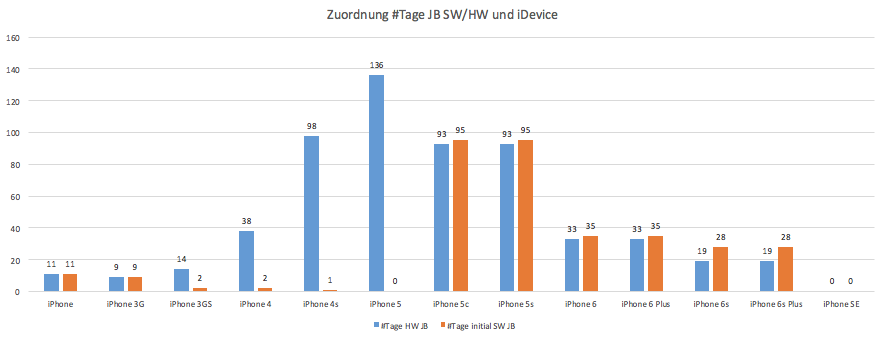
\includegraphics[scale=0.55]{Bilder/iDeviceJB-SW-HW.png}
         \caption{Vergleich der Anzahl der Tage eines JB für die Prozessoren und für der initialen iOS Version}
        \label{fig:VergleichJBProzessorSW}      
\end{figure}

Anhand der Abbildung \ref{fig:VergleichJBProzessorSW} kann gezeigt werden, dass alle Apple Prozessorarchitekturen einschliesslich der Apple A6 einen Sicherheitsgewinn für die iOS Produkte bedeutet haben. Da die JBs für diese iOS Version auf älteren Apple Prozessorarchitekturen innerhalb von wenigen Tagen verfügbar war. Ab der Apple Prozessorarchitektur A7 ist der Unterschied, zwischen dem veröffentlichen des JBs für die HW und die SW, nur mehr marginal. \par
\textbf{Dies lässt den Schluss zu, dass die Sicherheit und die Vertrauenswürdigkeit der iOS Produkte zum heutigen Zeitpunkt nur mehr vom mobilen Betriebssystem von Apple abhängt und nicht von der verwendeten iOS HW.}  

\begin{figure}[htbp]
        \centering
                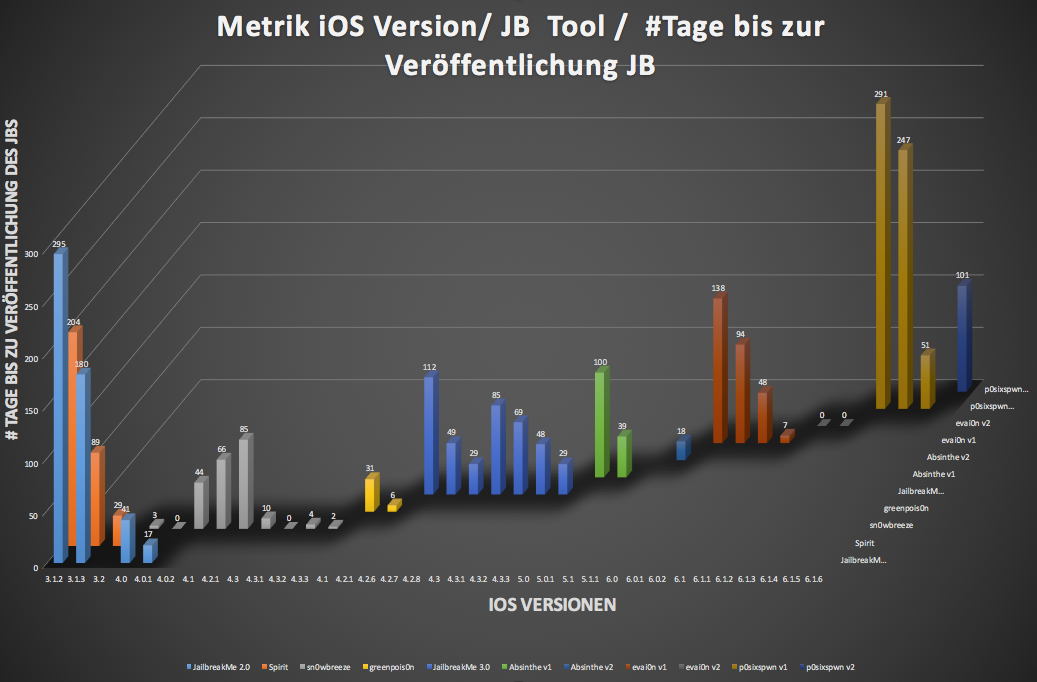
\includegraphics[scale=0.41]{Bilder/Frage1_1.png}
        \caption{iOS Version / JB Tools /\# Tage bis zum JB}
        \label{fig:AnalyseiOSJB1}        
\end{figure}

\begin{figure}[htbp]
        \centering
                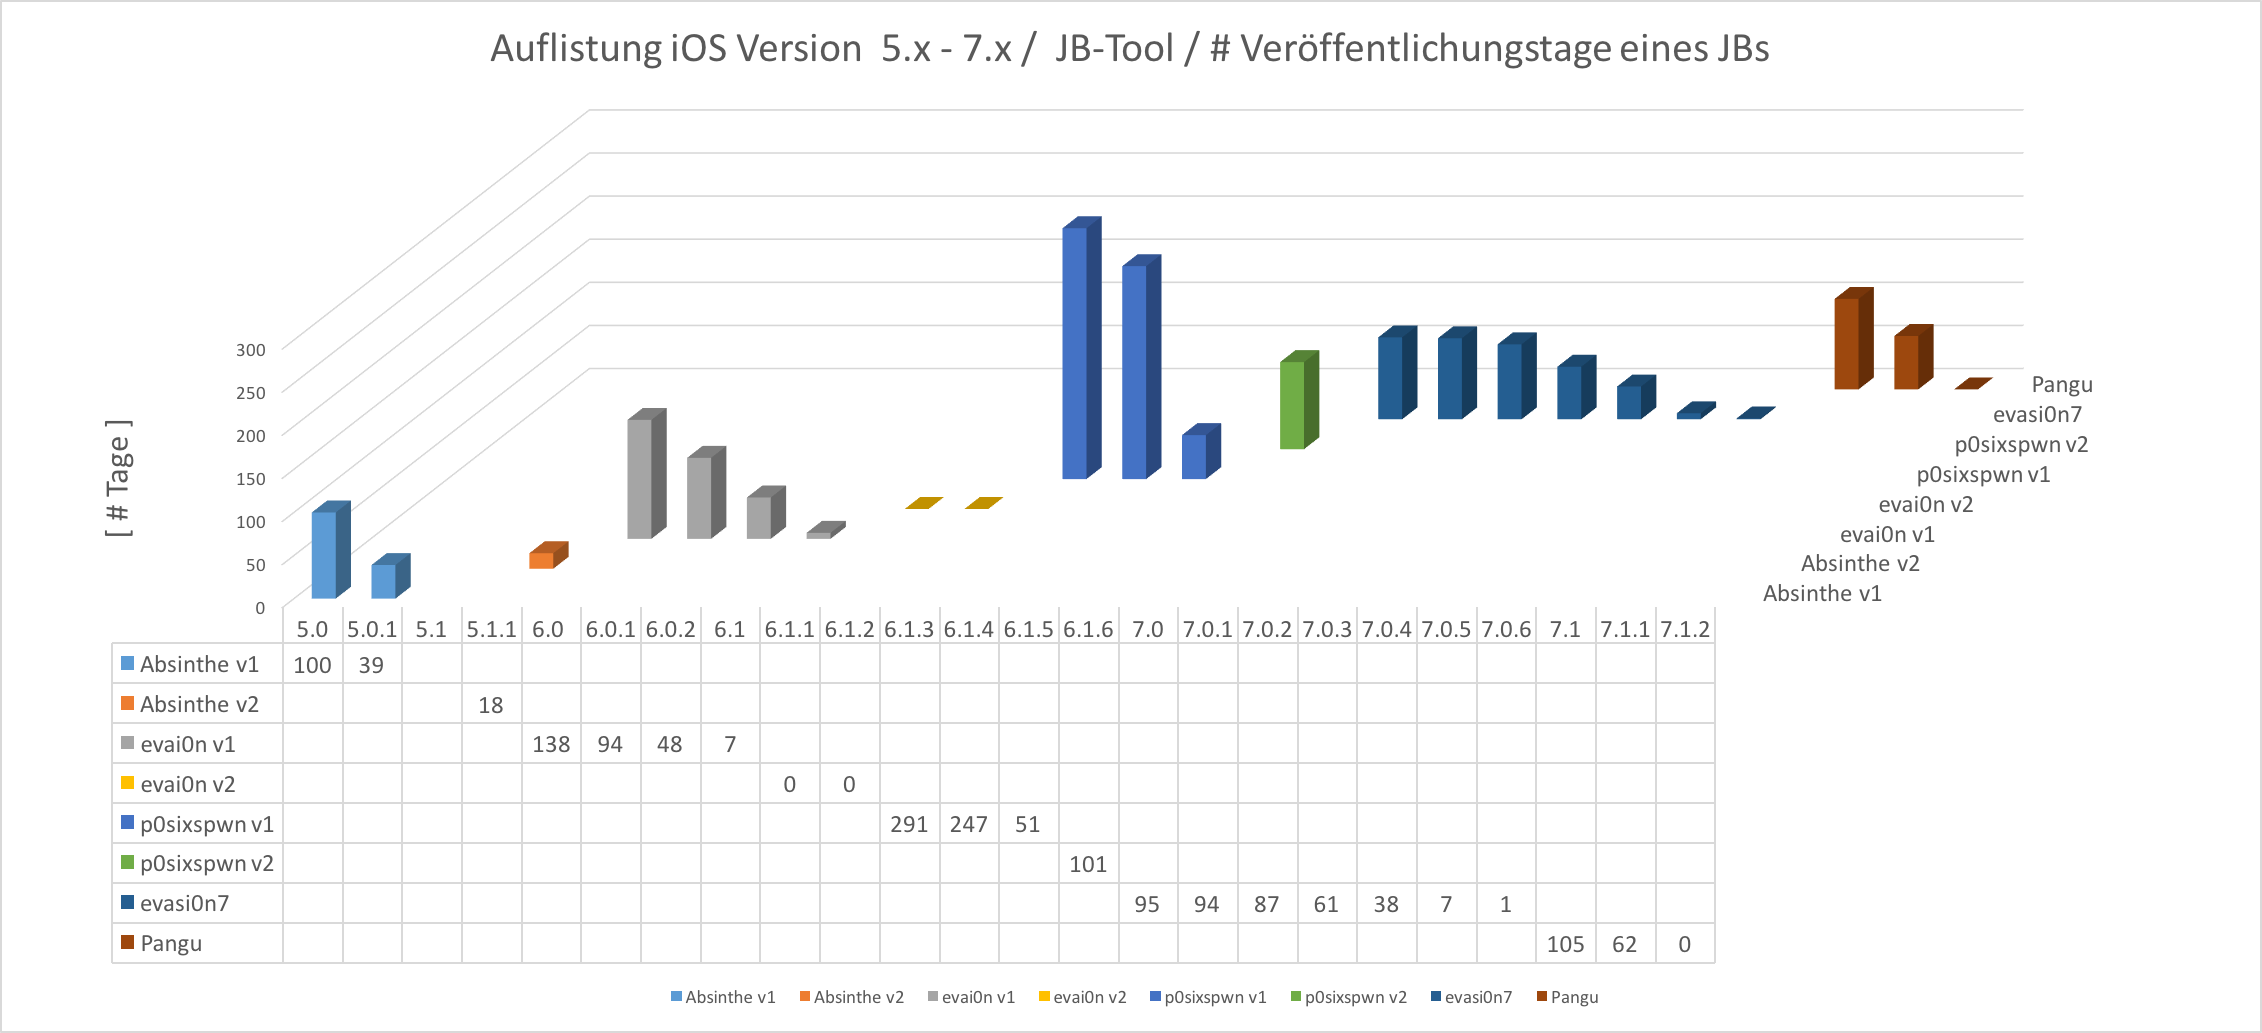
\includegraphics[scale=0.43]{Bilder/Frage1_2.png}
        \caption{iOS Version / JB Tools /\# Tage bis zum JB}
        \label{fig:AnalyseiOSJB2}
\end{figure}
Die Abbildungen \ref{fig:AnalyseiOSJB1} und \ref{fig:AnalyseiOSJB2} führen die bekanntesten untethered JBs an. Diese werden mit den iOS Versionen und der Anzahl an Tagen die benötigt wurden um das JB zu veröffentlichen in Verbindung gesetzt. 
\paragraph{Die Daten zeigen einerseits,} dass die Anzahl der veröffentlichten JB-Tool ab der iOS Version 7.0 massiv rückgängig sind. Es wurden nur mehr ein JB-Tool pro Major iOS Version der Öffentlichkeit zur Verfügung gestellt. Zudem sind ab der iOS Version nur mehr Teams die ein JBs veröffentlichen.
\paragraph{Anderseits zeigen die Daten,} dass nach einem gelungen JB die Sicherheitsupdates von Apple keinen Sicherheitsmehrwert mit sich bringen. Da innerhalb weniger Tage ein neuer JB des selben JB-Team veröffentlicht wurde. Dies gilt vor allem für alle iOS Versionen bis einschliesslich der iOS Version 7.x. Ab der iOS Version 8.x ändert sich dieses Verhalten. Markant ändern sich die Muster ab der iOS Version 9.x.

\section{Welche Auswirkung haben die von Apple eingeführten Sicherheitsmechanismen und Sicherheitsupdates auf die Sicherheit des Systems?}
\label{sec:Frage2}

            
     
\begin{description}
    \item[\parbox{\textwidth} {Antwort kurz INFO Katharina}]~\par
        \begin{itemize}
                \item Zuordnung Bugs / Sicherheitsmechanismen Ausreißer in den Stats Veröffentlichung \#Tage JB  
        \end{itemize}
\end{description} 
        




 